\documentclass[11pt, numbers=endperiod, parskip=half]{scrartcl}

\usepackage{amsmath}
\usepackage{graphicx}
\usepackage[final]{pdfpages}
\usepackage{pdflscape}
\usepackage{minted}
\usepackage{geometry}

\title{Assignment 8}
\subtitle{COS30023 - Languages in Software Development}
\author{Daniel Parker - 971328X}

\date{\today}

\begin{document}
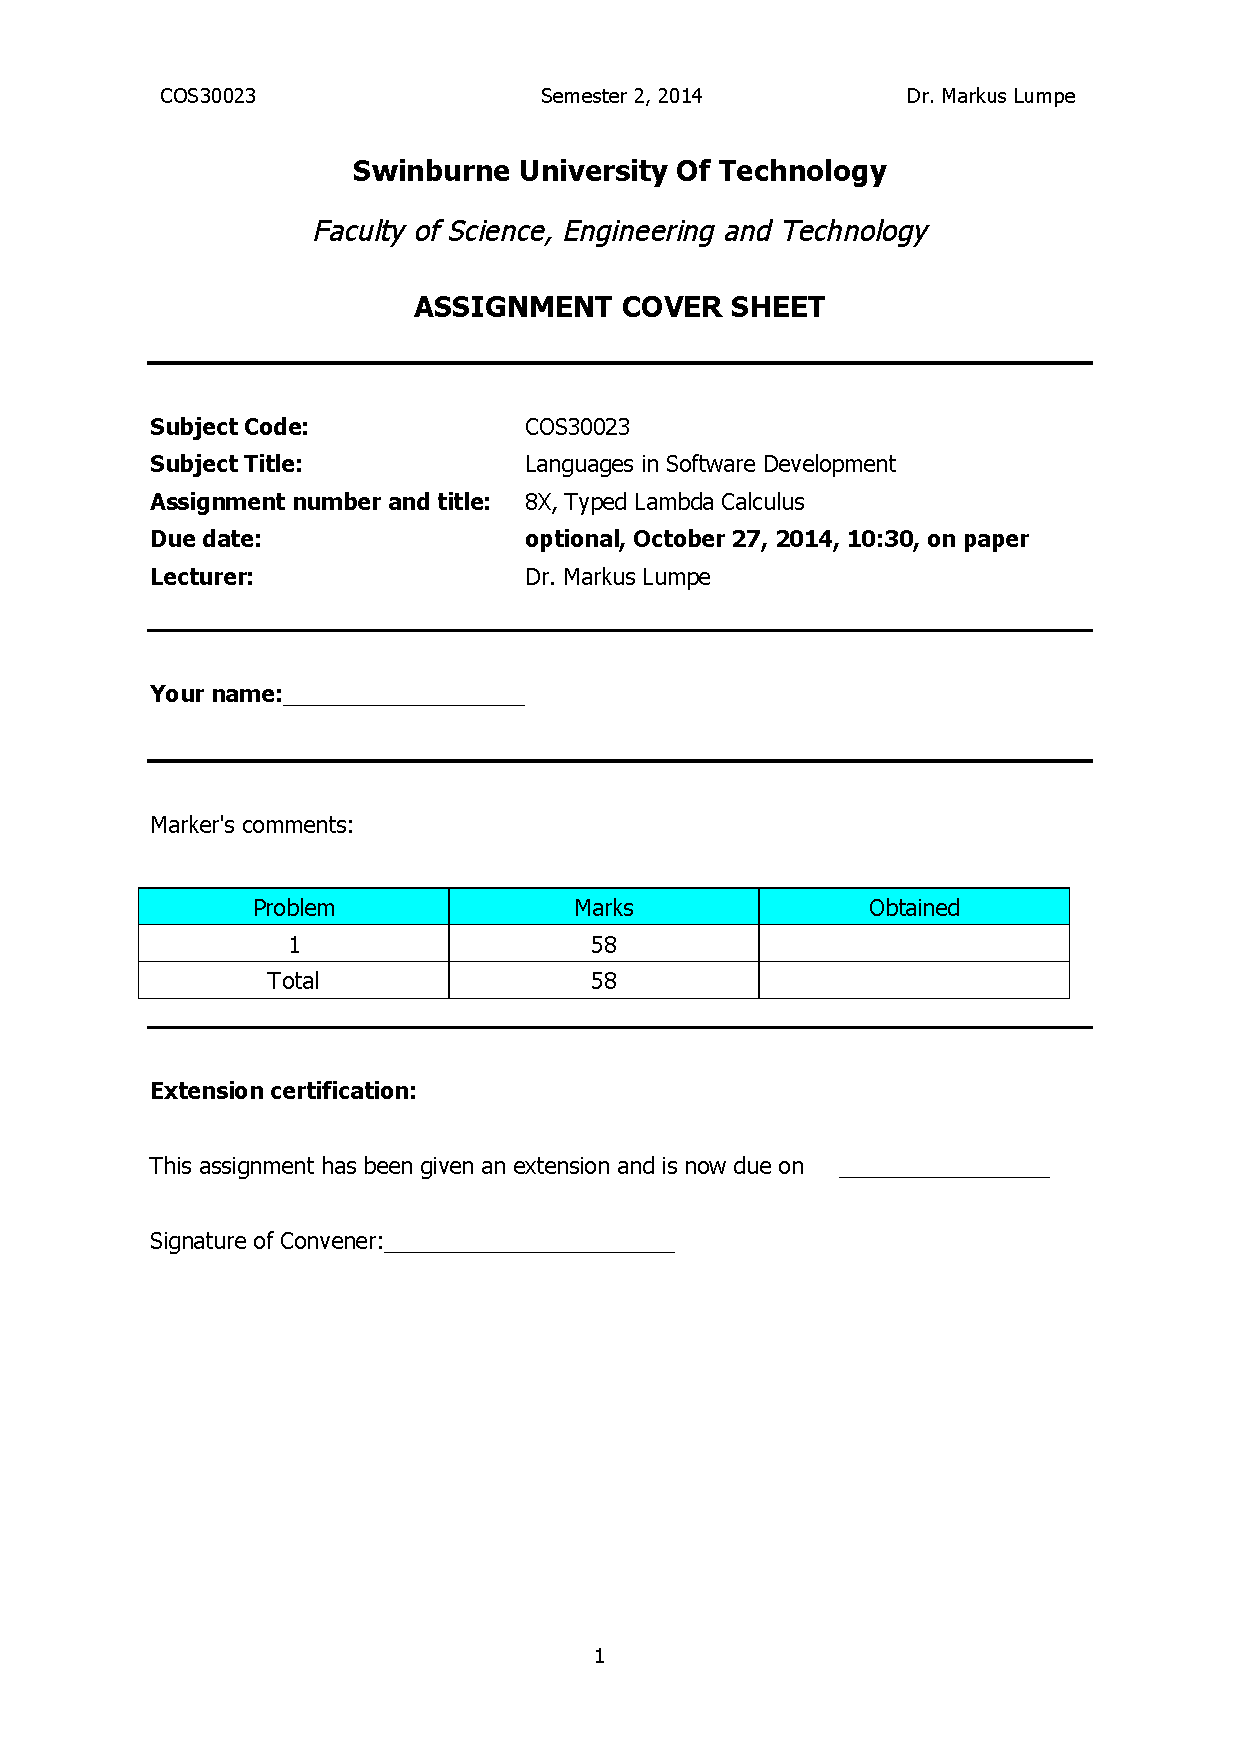
\includepdf[pages=1-1]{ProblemSet8.pdf}
\newgeometry{left=2.5cm}
\maketitle
% \begin{landscape}
\section{TypedLambda}
\subsection{TypedLambda.jj}
\inputminted[tabsize=2]{java}{LambdaTypeSystem/src/TypedLambda.jj}

\subsection{ast.TypedLambdaExpression}
\inputminted[tabsize=2]{java}{LambdaTypeSystem/src/ast/TypedLambdaExpression.java}

\subsection{ast.LambdaType}
\inputminted[tabsize=2]{java}{LambdaTypeSystem/src/ast/LambdaType.java}

\subsection{ast.IntegerType}
\inputminted[tabsize=2]{java}{LambdaTypeSystem/src/ast/IntegerType.java}

\subsection{ast.FunctionType}
\inputminted[tabsize=2]{java}{LambdaTypeSystem/src/ast/FunctionType.java}

\subsection{ast.LambdaNumber}
\inputminted[tabsize=2]{java}{LambdaTypeSystem/src/ast/LambdaNumber.java}

\subsection{ast.LambdaVariable}
\inputminted[tabsize=2]{java}{LambdaTypeSystem/src/ast/LambdaVariable.java}

\subsection{ast.LambdaFunction}
\inputminted[tabsize=2]{java}{LambdaTypeSystem/src/ast/LambdaFunction.java}

\subsection{ast.LambdaApplication}
\inputminted[tabsize=2]{java}{LambdaTypeSystem/src/ast/LambdaApplication.java}

\restoregeometry
\section{Results}
\subsection{error.lam}
\begin{minted}{scheme}
Checking: (lambda x (Int -> Int) .
            (lambda y (Int -> Int) . (lambda z Int . ((x z) (y z)))))
Oops, type error encountered: Function type expected for `(x z)'
\end{minted}
\subsection{one\_plus.lam}
\begin{minted}{scheme}
Checking: (((lambda m ((Int -> Int) -> (Int -> Int)) .
              (lambda n ((Int -> Int) -> (Int -> Int)) .
                (lambda s (Int -> Int) . (lambda z Int .
                  ((m s) ((n s) z))))))
                ((lambda n ((Int -> Int) -> (Int -> Int)) .
                  (lambda s (Int -> Int) . (lambda z Int . (s ((n s) z)))))
                (lambda s (Int -> Int) . (lambda z Int . z))))
                  ((lambda n ((Int -> Int) -> (Int -> Int)) .
                    (lambda s (Int -> Int) . (lambda z Int . (s ((n s) z)))))
                  (lambda s (Int -> Int) . (lambda z Int . z))))
SUCCESS: (((lambda m ((Int -> Int) -> (Int -> Int)) .
              (lambda n ((Int -> Int) -> (Int -> Int)) .
                (lambda s (Int -> Int) . (lambda z Int .
                  ((m s) ((n s) z))))))
                ((lambda n ((Int -> Int) -> (Int -> Int)) .
                  (lambda s (Int -> Int) . (lambda z Int . (s ((n s) z)))))
                (lambda s (Int -> Int) . (lambda z Int . z))))
                  ((lambda n ((Int -> Int) -> (Int -> Int)) .
                    (lambda s (Int -> Int) . (lambda z Int . (s ((n s) z)))))
                  (lambda s (Int -> Int) . (lambda z Int . z))))
has type ((Int -> Int) -> (Int -> Int))
\end{minted}
\end{document}
